%%%%%%%%%%%%%%%%%%%%%%%%%%%%%%  IEEEsample2e.tex %%%%%%%%%%%%%%%%%%%%%%%%%%%%%%
%% changes for IEEEtrans.cls marked with !PN
%% except all occ. of IEEEtran.sty changed IEEEtran.cls
%%%%%%%%%%                                                       %%%%%%%%%%%%%
%%%%%%%%%%    More information: see the header of IEEEtran.cls   %%%%%%%%%%%%%
%%%%%%%%%%                                                       %%%%%%%%%%%%%
%%%%%%%%%%%%%%%%%%%%%%%%%%%%%%%%%%%%%%%%%%%%%%%%%%%%%%%%%%%%%%%%%%%%%%%%%%%%%%%
\documentclass[journal]{IEEEtran} %!PN
%\documentclass[12pt,draft,onecolumn]{ieeetran} %!PN
%\documentstyle[twocolumn]{IEEEtran}
%\documentstyle[12pt,twoside,draft]{IEEEtran}
%\documentstyle[9pt,twocolumn,technote,twoside]{IEEEtran}
%\usepackage{epsfig}
\usepackage{amssymb}
\usepackage{epstopdf}
\usepackage{graphicx}
\usepackage{wrapfig}

\usepackage[english]{babel}
\usepackage[ansinew]{inputenc}

\usepackage{microtype,etex,listings,color,parskip}
\usepackage[margin=2cm]{geometry}
\usepackage{hyperref}

\usepackage{listings}
\usepackage{xcolor}

\usepackage{amsmath}
\usepackage{float}
%New colors defined below
\definecolor{backcolour}{rgb}{0.95,0.95,0.95}
\definecolor{codegreen}{rgb}{0,0.4,0.3}
\definecolor{codegray}{rgb}{0.5,0.5,0.5}
\definecolor{codepurple}{rgb}{0.58,0,0.82}
\definecolor{keywordcolour}{rgb}{0.1,0.3,0.7}

%Code listing style named "mystyle"
\lstdefinestyle{Python}{
  language=Python,
  basicstyle=\ttfamily\footnotesize,
  backgroundcolor=\color{backcolour},
  commentstyle=\color{codegreen},
  keywordstyle=\color{keywordcolour},
  numberstyle=\tiny\color{codegray},
  stringstyle=\color{codepurple},
  breakatwhitespace=false,         
  breaklines=true,                 
  captionpos=b,                    
  keepspaces=true,                 
  numbers=left,                    
  numbersep=5pt,
  showspaces=false,                
  showstringspaces=false,
  showtabs=false,                  
  tabsize=2
}

%"mystyle" code listing set
\lstset{style=Python}

%sets where to find graphics
\graphicspath{%
	{figs/}%
}

%maybe has to be changes
\usepackage{siunitx}
\sisetup{scientific-notation = true}%
%\sisetup{
%	locale = EN ,
%	per-mode = symbol,
%	separate-uncertainty,
%	range-phrase = --
%}

\setlength {\marginparwidth }{2cm}\usepackage{todonotes}

\usepackage{physics}


%%%%%%%%%%%%%%%%%
% Here it begins
%%%%%%%%%%%%%%%%%

\begin{document}

\title{Report 9 \\
Numerical solution of Bloch's equations for NMR}

%
\author{Lea Kanzleiter (402326), \href{mailto:lea.kanzleiter@gmx.de}{lea.kanzleiter@gmx.de}  \\
Tobias Rudolph (407229), \href{mailto:tobias.rudolph@rwth-aachen.de}{tobias.rudolph@rwth-aachen.de} \\
Date: 07.07.2020
}
%\thanks{The authors are with RWTH Aachen University, 52074 Aachen, Germany. Copyright (c) 2013 IEEE. Personal use of this material is permitted.
%However, permission to use this material for any other purposes must be
%obtained from the IEEE by sending a request to pubs-permissions@ieee.org.}}

\maketitle
%%%%%%%%%%%%%%%%%%%%%%%%%%%%%%%%%%%%%%%%%%%%%%%%%%%%%%%%%%%%%%%%%%%%%%%%
\begin{abstract}
This report presents a simulation of the nuclear magnetic resonance phenomenon. A numeric solution to Bloch's equations for the interdependence of the magnetic field and the system magnetization was implemented and the time evolution of the magnetization was observed.
\end{abstract}

%\begin{IEEEkeywords}
%...,...,... .
%\end{IEEEkeywords}


\section{Introduction}\label{intro}
\IEEEPARstart{I}{n} 1946, Bloch proposed a set of macroscopic differential equations, which characterize the time-dependent behaviour of a system's bulk magnetization in an external magnetic field. The model is based on the assumption of non-interacting nuclei with spin $\frac{1}{2}$. In general, the interdependence of the bulk magnetization $\mathbf{M}(t)$ and the magnetic field $\mathbf{B}(t)$ is given as:
\begin{equation}
    \frac {d \mathbf {M}(t)} {d t} = \gamma  \mathbf {M} (t) \times \mathbf {B} (t)
\end{equation}
Here, $\gamma$ is the gyromagnetic ratio.
An important mechanism in \textbf{nuclear magnetic resonance (NMR)} experiments is the spin relaxation, which can be classified in two different processes. The first is \textbf{longitudinal relaxation}, determined by the relaxation time constant $\frac{1}{T_1}$. It describes the return of the magnetization's longitudinal component to its equilibrium value. Since it is based on the realignment of the spins with the initial magnetic field, it is also called \textbf{Spin-Lattice-Relaxation}.
The second process is the \textbf{transverse relaxation}, characterized by the time constant $\frac{1}{T_2}$.
It describes the decay of the transverse magnetization component. Considering the relaxation processes and separating the spatial coordinates, the magnetization is defined by:

\begin{align}
\frac {d M_x(t)} {d t} &= \gamma ( \mathbf {M} (t) \times \mathbf {B} (t)  )_x - \frac {M_x(t)} {T_2} \\
\frac {d M_y(t)} {d t} &= \gamma ( \mathbf {M} (t) \times \mathbf {B} (t)  )_y - \frac {M_y(t)} {T_2} \\
\frac {d M_z(t)} {d t} &= \gamma ( \mathbf {M} (t) \times \mathbf {B} (t)  )_z - \frac {M_z(t) - M_0} {T_1} \label{eq:3}
\end{align}

The external magnetic field the nuclei are exposed to can be written as:
\begin{align}
    \mathbf{B}(t) = (B_x(t),\, B_y(t),\, B_0 + \Delta B_z(t))
\end{align}
The $z$ component of the magnetic field $\mathbf{B}(t)$ is composed of a constant term $B_0$, and a time-dependent term $\Delta B_z(t)$. $B_z(t)$ is the basis for spatial decoding of the NMR signal in magnetic resonance imaging (MRI). In equation \eqref{eq:3}, $M_0$ denotes the steady state magnetization for the time limit $t \rightarrow \infty$. In this report, it is assumed to be zero.


%\todo{Rabi Oscillation}
%Rabi oscillations
%One can turn the spin by applying a microwave pulse $ M_z (t) = -M_z(0)$.
%One can put the magnetization in the x-y plane if one chooses $\gamma h t = \pi / 2$  $ M_z (t) = -M_z(t = 0) %$

\section{Simulation model and method}
For the simulation, the correct choice of time steps $\tau$ is crucial since the magnetic field B is overall not constant in time. It is however sufficient to assume a constant field within one time step, if $\tau$ is chosen small enough. This results in the following equation for the time evolution of the magnetization vector:
\begin{equation}
    \mathbf{M}(t+\tau) = \exp(\tau \gamma \mathbf{B}(t+ \tau/2)) \, \mathbf{M}(t)
\end{equation}
Starting with an initial magnetization $\textbf{M}(0)$, the value at the time t can be obtained by repeatedly applying the time evolution matrix $e^{\tau \gamma \mathbf{B}}$:
\begin{align}
    \mathbf{M}(t)= e^{\tau \gamma \mathbf{B}(t-\tau/2)} \, e^{\tau \gamma \mathbf{B}(t-3\tau/2)}\, ....\, e^{\tau \gamma \mathbf{B}(\tau/2)}\mathbf{M}(0)
\end{align}
Since $\tau$ was chosen sufficiently small, the solution for $\textbf{B} = const.$ can be used here.

In order to incorporate both relaxation processes, a diagonal matrix C containing the time constants $T_1$ and $T_2$ is added to the magnetic field matrix used in the simulation.

\begin{equation}
    B \rightarrow B + C
\end{equation}

\begin{align}
C = -
\begin{pmatrix}
1/\gamma T_2 & 0 & 0  \\
0 & 1/\gamma T_2 & 0 \\
0 & 0 & 1/\gamma T_1 \\
\end{pmatrix}
\end{align}

\begin{align}
e^{\tau\gamma C/2} = 
\begin{pmatrix}
e^{-\tau/2 T_2} & 0 & 0  \\
0 & e^{-\tau/2 T_2} & 0 \\
0 & 0 & e^{-\tau/2 T_1} \\
\end{pmatrix}
\end{align}

Including this update to the magnetic field matrix B, the time evolution of the magnetization vector is calculated with the new factor:
\begin{align}
    e^{\tau \gamma B} \longrightarrow e^{\tau \gamma C/2} e^{\tau \gamma B} e^{\tau \gamma C/2} 
\end{align}

The magnetic field used for the simulations in this report is composed as follows:
\begin{align}
\mathbf{B}(t) = \begin{pmatrix}h \cos(\omega_0 t) \\\ -h \sin(\omega_0 t) \\\ B_0 \end{pmatrix}    
\end{align}
Here, $\omega_0$ is the Larmor precession frequency. It is induced by the interaction of the magnetization component that is perpendicular to the magnetic field and the field itself. The resulting torque on the perpendicular component results in the precession with the frequency $\omega_0$.

The remaining system parameters were set to:
\begin{align*}
    B_0 &= 2 \pi f_0 \,\,\text{with}\,\, f_0 = 4 \\
    h &= 2 \pi f_1 \,\, \text{with}\,\, f_1 = \frac{1}{4}\\
    \gamma &= 1 \\
    \omega_0 &= B_0 \\
    \tau &= 0.01
\end{align*}


\section{Simulation results}
The simulation was carried out for different combinations of relaxation time constants $\frac{1}{T_1}$, $\frac{1}{T_2}$ and initial magnetizations. For each simulation run, 100 steps were used to resolve $f_0$, before the time evolution was observed.\newline
Figure \ref{f0} contains the results for\footnote{Note that we plotted the magnetization and therefore the $y$-axis is in the unit of a magnetization.}:
\begin{align}
    \frac{1}{T_1} = 0, \frac{1}{T_2} = 0, \mathbf{M}(t=0) = (0, 1, 0)
\end{align}
\begin{figure}[H]
\centering
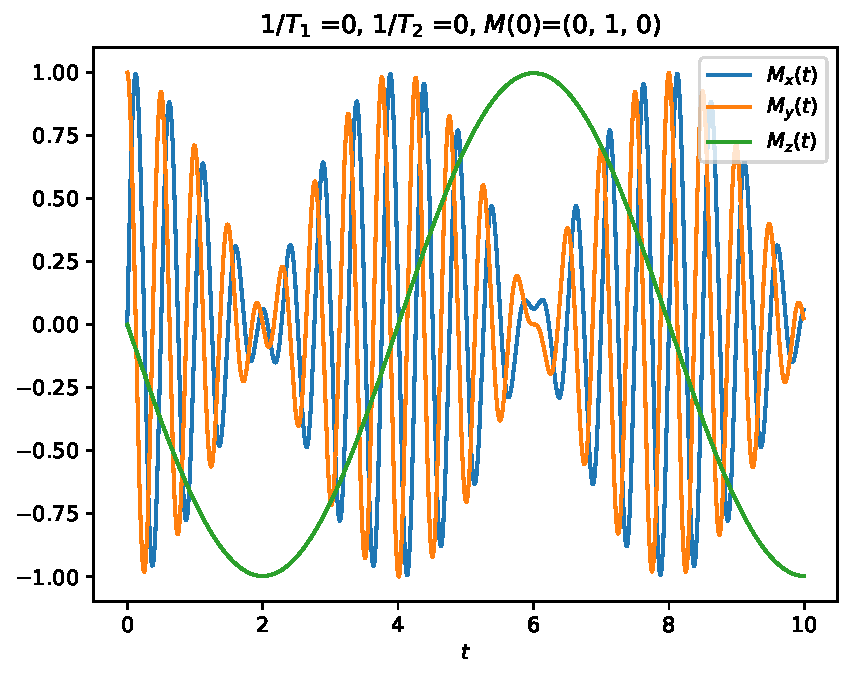
\includegraphics[width=2.5in]{NMR_T1-0_T2-0_Minit-010_tau_0.01_t_10.pdf}
\caption{Time evolution of the bulk magnetization components for $1/T_1 = 0$, $1/T_2 = 0$, M(t=0) = (0, 1, 0), $\phi = 0$}
\label{f0}
\end{figure}
Since in this case, no relaxation occurs. The plot shows, that the oscillations are not damped, which matches the theory. It also shows, that the $z$-component of the magnetization oscillates with a significantly lower frequency than the $x$- and $y$-components.

The plot in figure \ref{f1} shows the results for:
\begin{align}
    \frac{1}{T_1} = 1, \frac{1}{T_2} = 0, \mathbf{M}(t=0) = (0, 1, 0)
\end{align}
\begin{figure}[H]
\centering
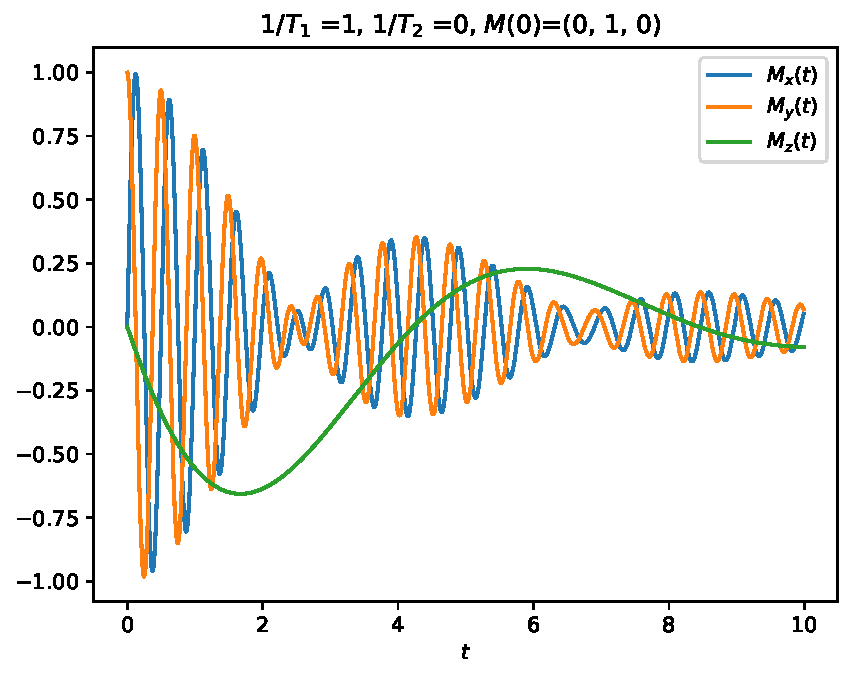
\includegraphics[width=2.5in]{figs/NMR_T1-1_T2-0_Minit-010_tau_0.01_t_10_no_phase.pdf}
\caption{Time evolution of the bulk magnetization components for $1/T_1 = 1$, $1/T_2 = 0$, M(t=0) = (0, 1, 0), $\phi = 0$}
\label{f1}
\end{figure}
When adding a $\frac{1}{T_1}$ relaxation, the amplitudes of the $M_z$-oscillations, as well as the maximum amplitude of the $M_x$ and $M_y$ wave packets are damped and enveloped by an exponential function.

The next plot (figure \ref{f2}) shows the magnetization for:
\begin{align}
    \frac{1}{T_1} = 0, \frac{1}{T_2} = 1, \mathbf{M}(t=0) = (0, 1, 0)
\end{align}
\begin{figure}[H]
\centering
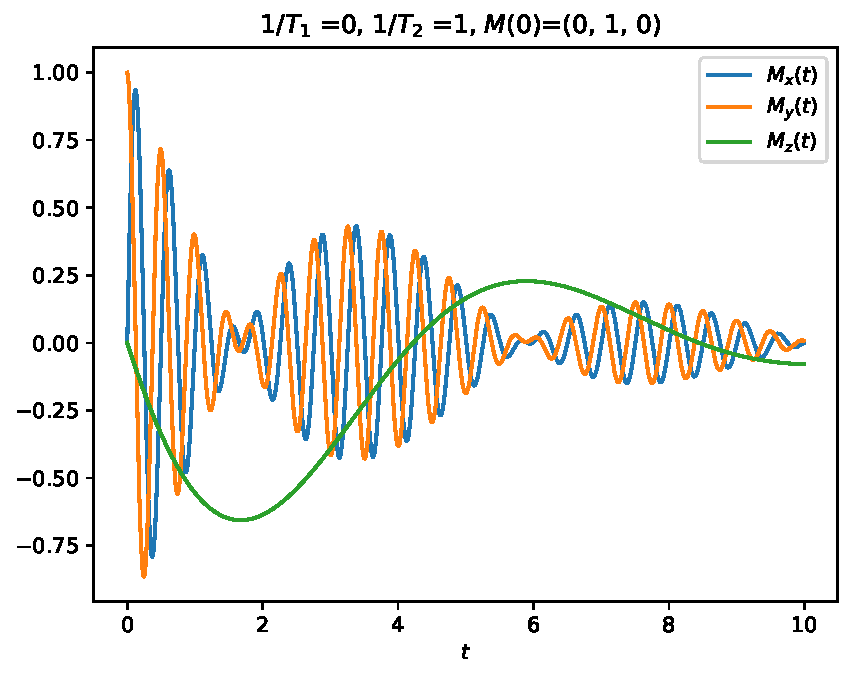
\includegraphics[width=2.5in]{figs/NMR_T1-0_T2-1_Minit-010_tau_0.01_t_10_no_phase.pdf}
\caption{Time evolution of the bulk magnetization components for $1/T_1 = 0$, $1/T_2 = 1$, M(t=0) = (0, 1, 0), $\phi = 0$}
\label{f2}
\end{figure}
In the case of only $\frac{1}{T_2}$ relaxation, a similar behaviour can be observed. However, the amplitudes magnetization oscillations are damped more slowly. 


In figure \ref{f3}, the magnetization was plotted for:
\begin{align}
    \frac{1}{T_1} = 1, \frac{1}{T_2} = 1, \mathbf{M}(t=0) = (0, 1, 0)
\end{align}
\begin{figure}[H]
\centering
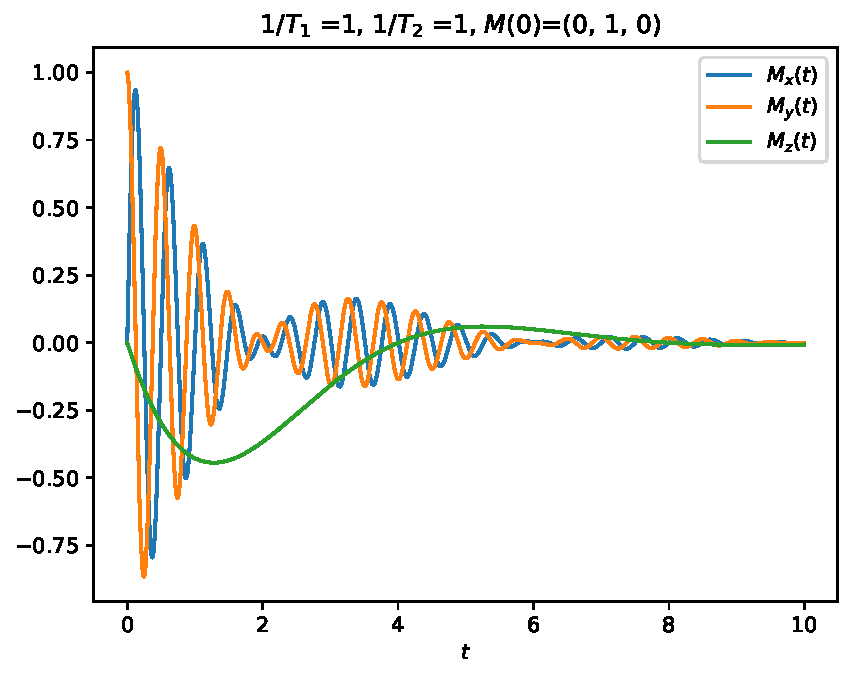
\includegraphics[width=2.5in]{figs/NMR_T1-1_T2-1_Minit-010_tau_0.01_t_10_no_phase.pdf}
\caption{Time evolution of the bulk magnetization components for $1/T_1 = 1$, $1/T_2 = 1$, M(t=0) = (0, 1, 0), $\phi = 0$}
\label{f3}
\end{figure}
As expected, the damping according to the exponential function is much stronger, if both relaxations are present. This can easily be seen in figure \ref{f3}.


To observe the behaviour of the magnetization more detailed, a phase $\phi$ was introduced to the magnetic field:
\begin{align}
\mathbf{B}(t) = \begin{pmatrix}h \cos(\omega_0 t + \phi) \\\ -h \sin(\omega_0 t + \phi) \\\ B_0 \end{pmatrix}    
\end{align}

The time evolution was calculated and plotted for the phases
\begin{align*}
    \phi &= \frac{\pi}{2} \\
    \phi &= \frac{\pi}{4}
\end{align*}
in combination with three different initial orientations $\textbf{M}(0)$ of the magnetization:
\begin{align}
    \mathbf{M}(t=0) &= (1, 0, 0) \\
                    &= (0, 0, 1) \\
                    &= (1, 0, 1)
\end{align}
The results can be found in figures \ref{f4} through \ref{f9}.

Firstly, the results for the phase \textbf{$\phi = \frac{\pi}{2}$} are presented. For the relaxation times
\begin{align}
    \frac{1}{T_1} = 1, \frac{1}{T_2} = 0,
\end{align}
the plots for the three different initial magnetizations are in figures \ref{f4} through \ref{f6}.

\begin{figure}[H]
\centering
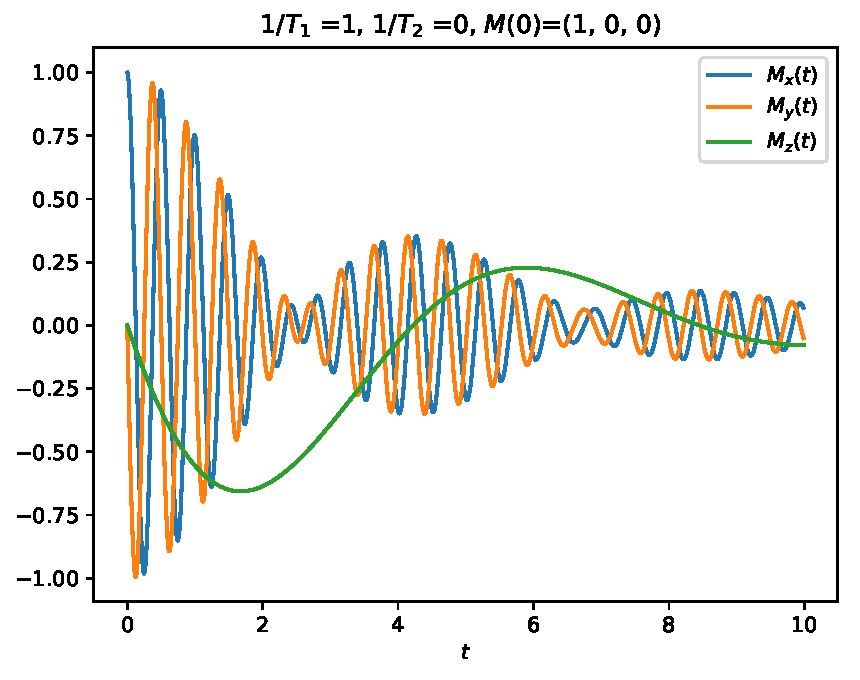
\includegraphics[width=2.5in]{figs/NMR_T1-1_T2-0_Minit-100_tau_0.01_t_10_phase_pi_2.pdf}
\caption{Time evolution of the bulk magnetization components for $1/T_1 = 1$, $1/T_2 = 0$, M(t=0) = (1, 0, 0), $\phi = \frac{\pi}{2}$}
\label{f4}
\end{figure}
In figure \ref{f4}, the z-component is zero at the time t=0, while the amplitude for the x- and y-components is at its maximum at the same time. This shows, that the phase shift $\phi$ was only applied to the x- and y-components of the magnetic field. The same can be observed in the next plot (figure \ref{f5}). However, the z-component is at its maximum at t=0, since the initial magnetization was chosen to be in z-direction contrary to plot \ref{f4}.
\begin{figure}[H]
\centering
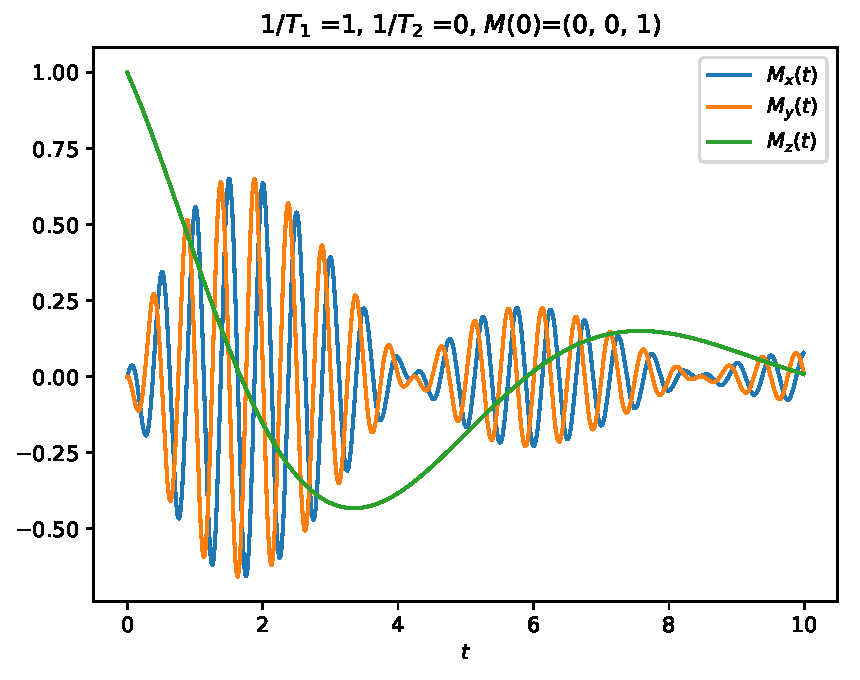
\includegraphics[width=2.5in]{figs/NMR_T1-1_T2-0_Minit-001_tau_0.01_t_10_phase_pi_2.pdf}
\caption{Time evolution of the bulk magnetization components for $1/T_1 = 1$, $1/T_2 = 0$, M(t=0) = (0, 0, 1), $\phi = \frac{\pi}{2}$}
\label{f5}
\end{figure}

\begin{figure}[H]
\centering
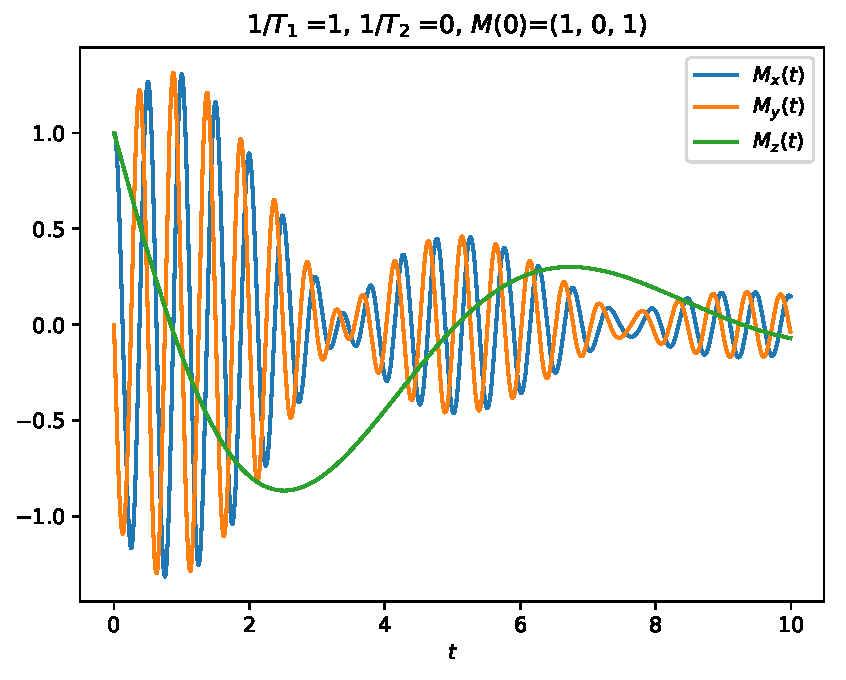
\includegraphics[width=2.5in]{figs/NMR_T1-1_T2-0_Minit-101_tau_0.01_t_10_phase_pi_2.pdf}
\caption{Time evolution of the bulk magnetization components for $1/T_1 = 1$, $1/T_2 = 0$, M(t=0) = (1, 0, 1), $\phi = \frac{\pi}{2}$}
\label{f6}
\end{figure}



For the phase $\phi = \frac{\pi}{4}$, and the relaxation time constants
\begin{align}
    \frac{1}{T_1} = 1, \frac{1}{T_2} = 0,
\end{align}
the results can be found in figures \ref{f7} through \ref{f9}.
\begin{figure}[H]
\centering
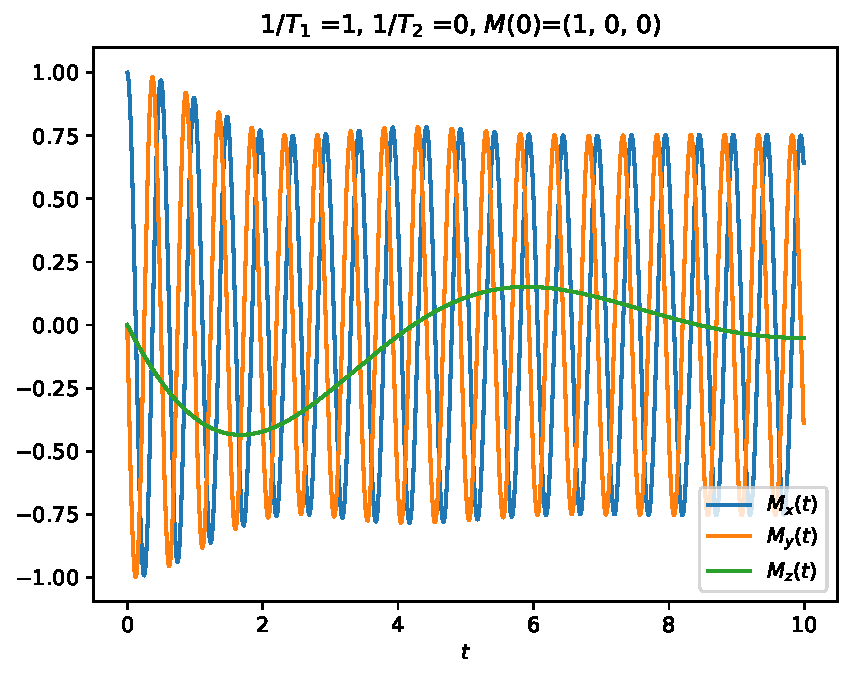
\includegraphics[width=2.5in]{figs/NMR_T1-1_T2-0_Minit-100_tau_0.01_t_10_phase_pi_4.pdf}
\caption{Time evolution of the bulk magnetization components for $1/T_1 = 1$, $1/T_2 = 0$, M(t=0) = (1, 0, 0), $\phi = \frac{\pi}{4}$}
\label{f7}
\end{figure}
Analog to the observations for $\phi = \frac{\pi}{2}$, the plots for $\phi = \frac{\pi}{4}$ show the phase shift as expected.
\begin{figure}[H]
\centering
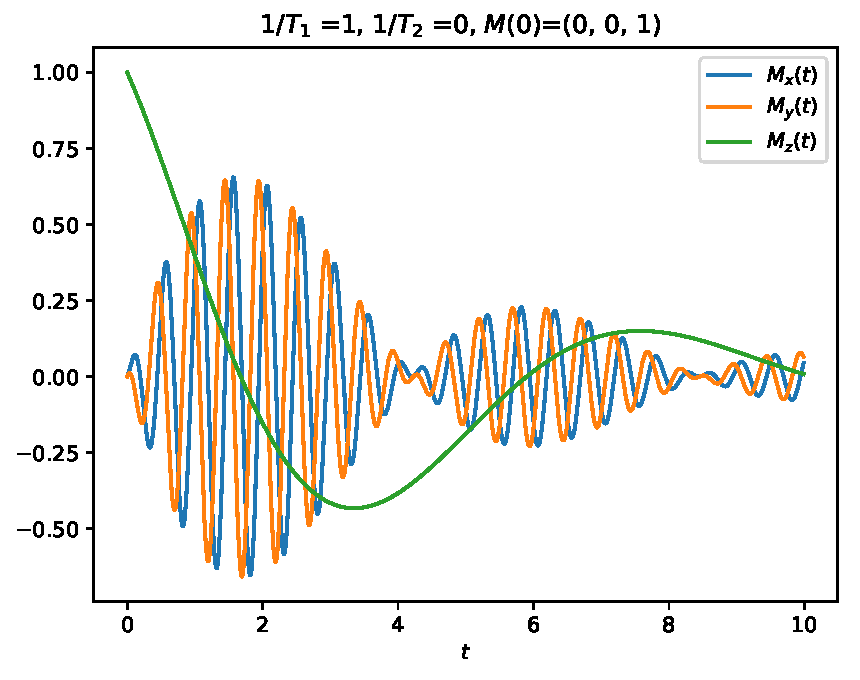
\includegraphics[width=2.5in]{figs/NMR_T1-1_T2-0_Minit-001_tau_0.01_t_10_phase_pi_4.pdf}
\caption{Time evolution of the bulk magnetization components for $1/T_1 = 1$, $1/T_2 = 0$, M(t=0) = (0, 0, 1), $\phi = \frac{\pi}{4}$}
\label{f8}
\end{figure}
\begin{figure}[H]
\centering
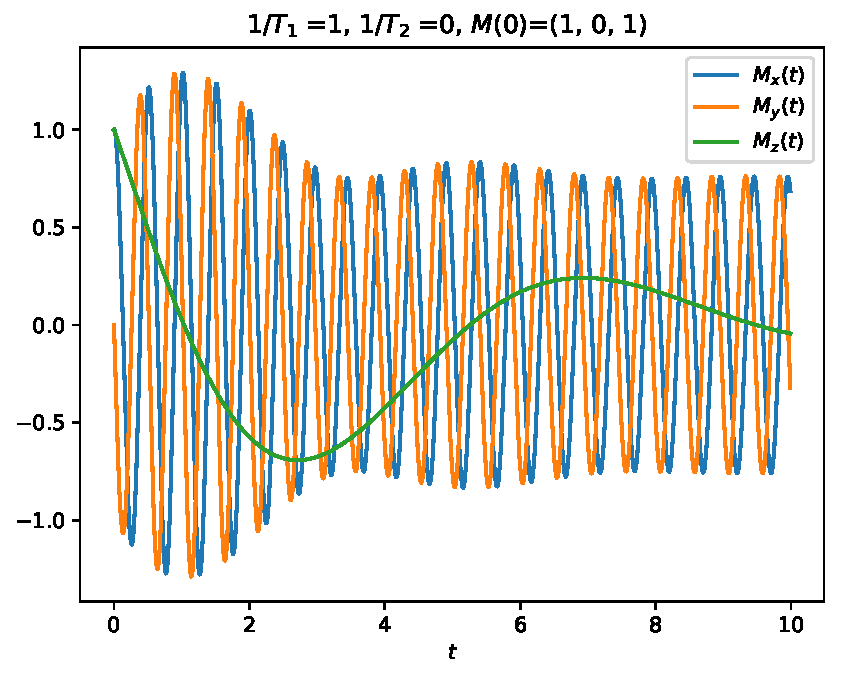
\includegraphics[width=2.5in]{figs/NMR_T1-1_T2-0_Minit-101_tau_0.01_t_10_phase_pi_4.pdf}
\caption{Time evolution of the bulk magnetization components for $1/T_1 = 1$, $1/T_2 = 0$, M(t=0) = (1, 0, 1), $\phi = \frac{\pi}{4}$}
\label{f9}
\end{figure}
In figure \ref{f9}, the phase shift can be seen quite well at the time $t=0$. Neither the $z$- nor the $x$- and $y$-components are at either zero or their maximum. Since the initial magnetization was a linear combination of $x$- and $z$-components, the damping is not as fast as in the previous plots.  

\begin{figure}[H]
\centering
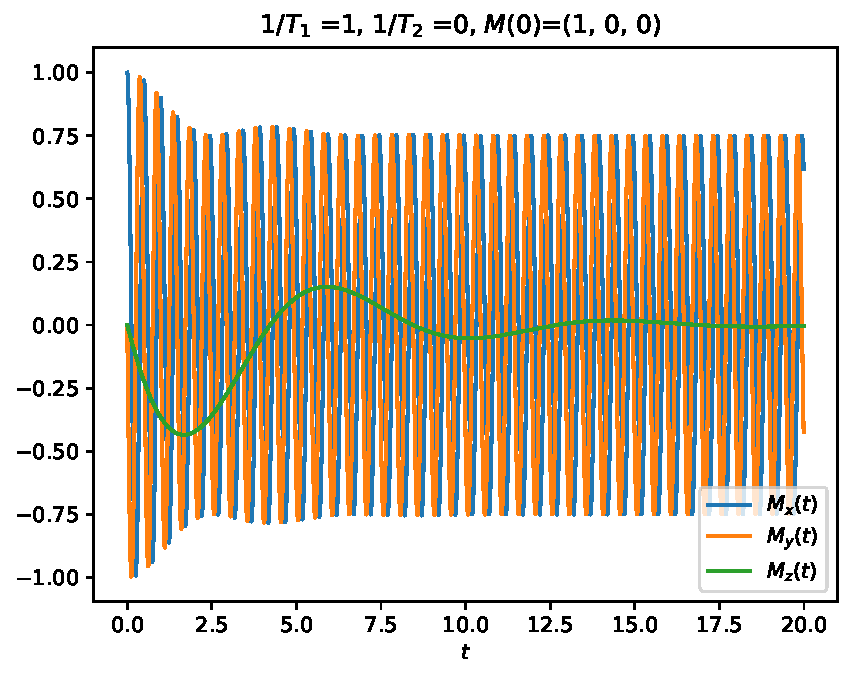
\includegraphics[width=2.5in]{figs/NMR_T1-1_T2-0_Minit-100_tau_0.01_t_20.pdf}
\caption{Time evolution of the bulk magnetization components for $1/T_1 = 1$, $1/T_2 = 0$, M(t=0) = (1, 0, 1), $\phi = \frac{\pi}{4}$ for a longer time.}
\label{flonger}
\end{figure}
In addition to figure \ref{f9}, the same setup was analyzed for a longer time period. In conclusion, the amplitude of the oscillation decays slower than in the other configurations.   

The results for the remaining combinations of phases, initial magnetization and relaxation time constants can be found in the appendix (compare figures \ref{f10} through \ref{f21}).

\section{Discussion}

With the product formula approach we were able to solve the Bloch equation numerically and we observed the evolution of the magnetization over time exposed to a magnetic field. The influence from the relaxation time constants $\frac{1}{T_1}$ and $\frac{1}{T_2}$ is as expected.  

%%%%%%%%%%%%%%%%%%%%%%%%%%%%%%%%%%%%%%%%%%%%%%%%%%%%%%%%%%%%%%%%%%%%%%%%%%%%%%%%%%%%%%%%%%%%%%%%%%%%%%%%%%%%
%%%%%%%%%%%%%%%%%%%%%%%%%%%%%%%%%%%%%%%%%%%%%%%%%%%%%%%%%%%%%%%%%%%%%%%%%%%%%%%%%%%%%%%%%%%%%%%%%%%%%%%%%
%To have the Appendix on a new page, but can also be deleted
\clearpage

\section*{Appendix}
Results for phase $\phi = \frac{\pi}{2}, \frac{1}{T_1} = 0, \frac{1}{T_2} = 1$:
\begin{figure}[H]
\centering
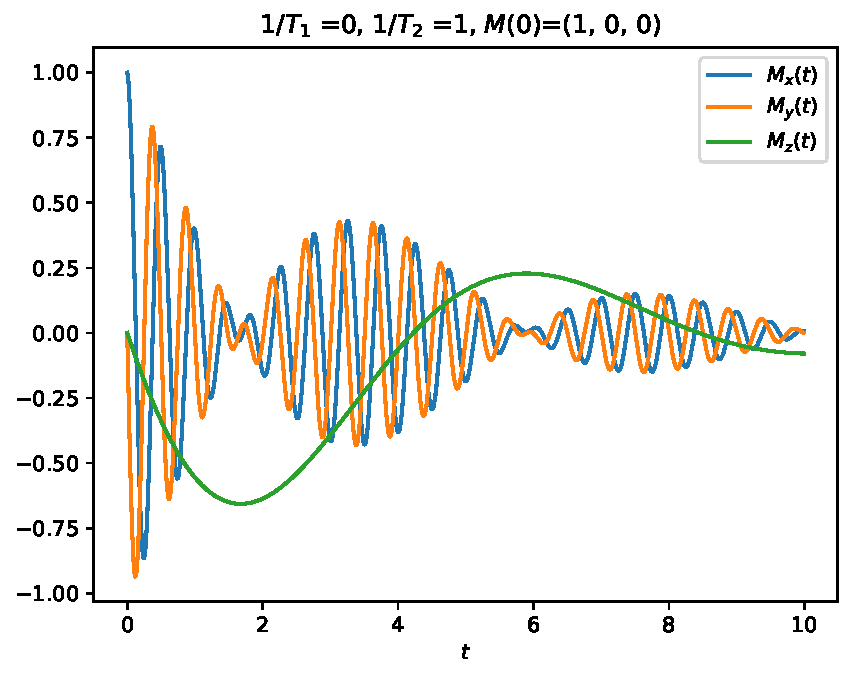
\includegraphics[width=2.5in]{figs/NMR_T1-0_T2-1_Minit-100_tau_0.01_t_10_phase_pi_2.pdf}
\caption{Time evolution of the bulk magnetization components for $1/T_1 = 0$, $1/T_2 = 1$, M(t=0) = (1, 0, 0), $\phi = \frac{\pi}{2}$}
\label{f10}
\end{figure}
\begin{figure}[H]
\centering
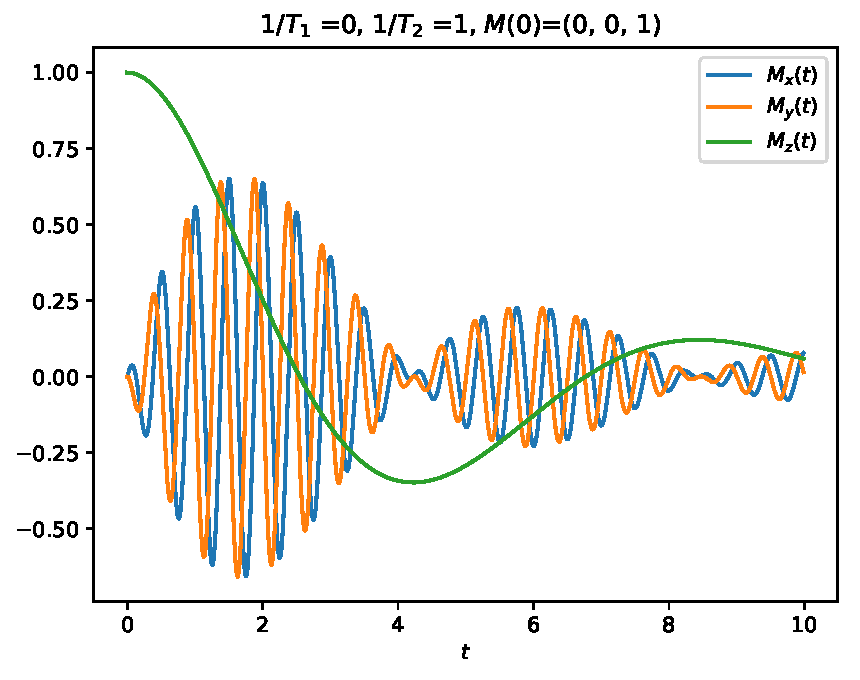
\includegraphics[width=2.5in]{figs/NMR_T1-0_T2-1_Minit-001_tau_0.01_t_10_phase_pi_2.pdf}
\caption{Time evolution of the bulk magnetization components for $1/T_1 = 0$, $1/T_2 = 1$, M(t=0) = (0, 0, 1), $\phi = \frac{\pi}{2}$}
\label{f11}
\end{figure}
\begin{figure}[!htb]
\centering
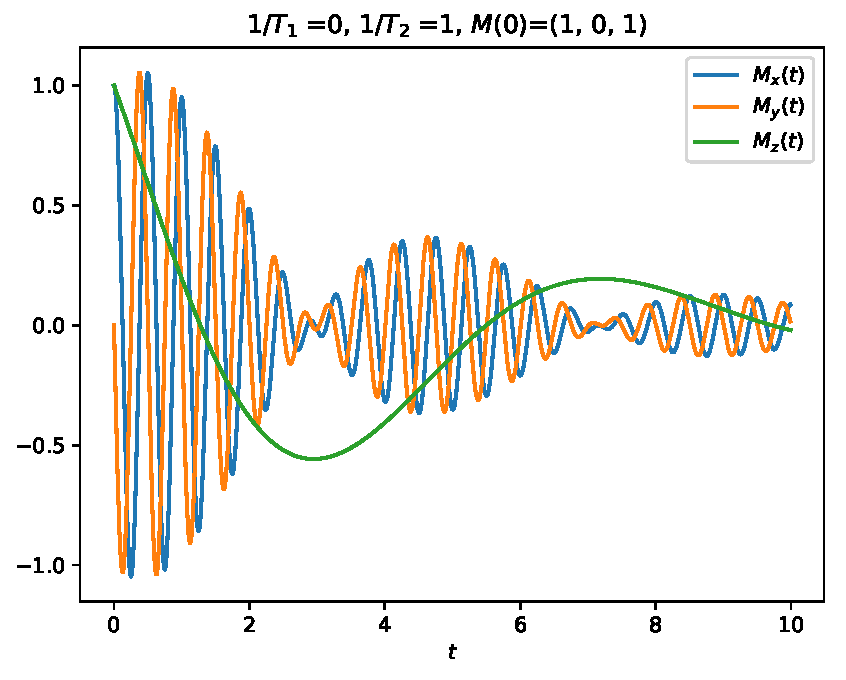
\includegraphics[width=2.5in]{figs/NMR_T1-0_T2-1_Minit-101_tau_0.01_t_10_phase_pi_2.pdf}
\caption{Time evolution of the bulk magnetization components for $1/T_1 = 0$, $1/T_2 = 1$, M(t=0) = (1, 0, 1), $\phi = \frac{\pi}{2}$}
\label{f12}
\end{figure}
\newpage

Results for phase $\phi = \frac{\pi}{2}, \frac{1}{T_1} = 1, \frac{1}{T_2} = 1$:
\begin{figure}[H]
\centering
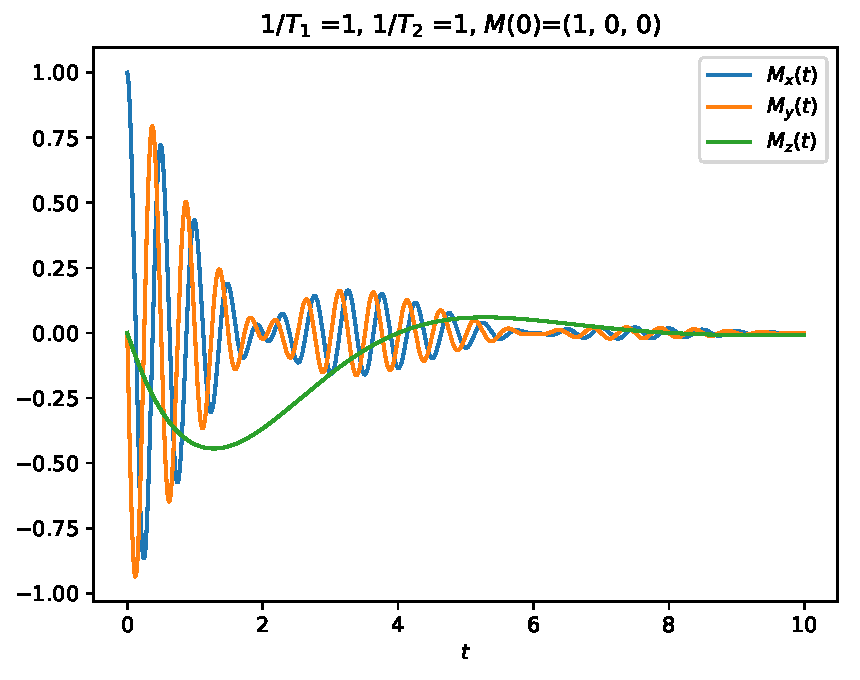
\includegraphics[width=2.5in]{figs/NMR_T1-1_T2-1_Minit-100_tau_0.01_t_10_phase_pi_2.pdf}
\caption{Time evolution of the bulk magnetization components for $1/T_1 = 1$, $1/T_2 = 1$, M(t=0) = (1, 0, 0), $\phi = \frac{\pi}{2}$}
\label{f13}
\end{figure}
\begin{figure}[H]
\centering
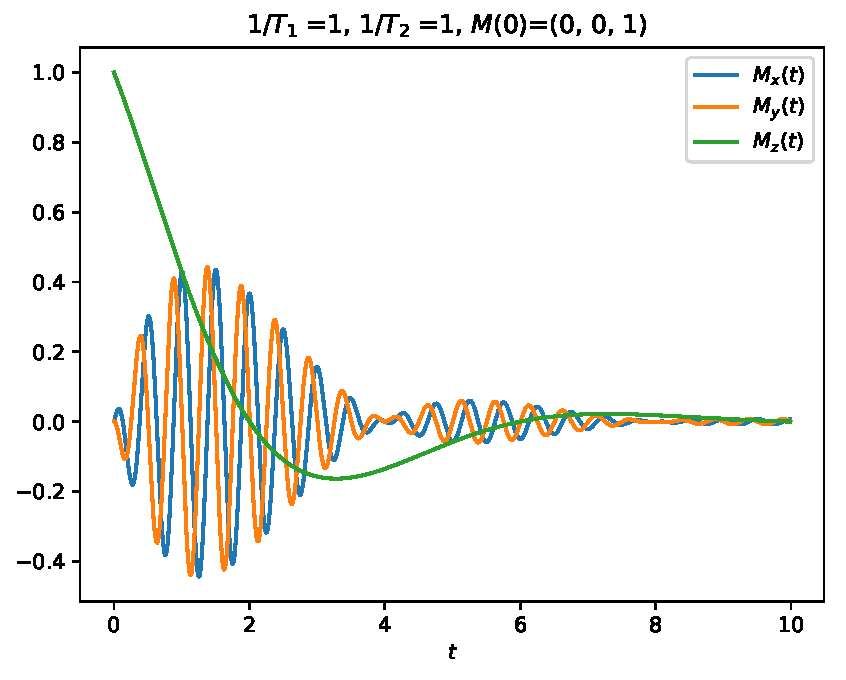
\includegraphics[width=2.5in]{figs/NMR_T1-1_T2-1_Minit-001_tau_0.01_t_10_phase_pi_2.pdf}
\caption{Time evolution of the bulk magnetization components for $1/T_1 = 1$, $1/T_2 = 1$, M(t=0) = (0, 0, 1), $\phi = \frac{\pi}{2}$}
\label{f14}
\end{figure}
\begin{figure}[H]
\centering
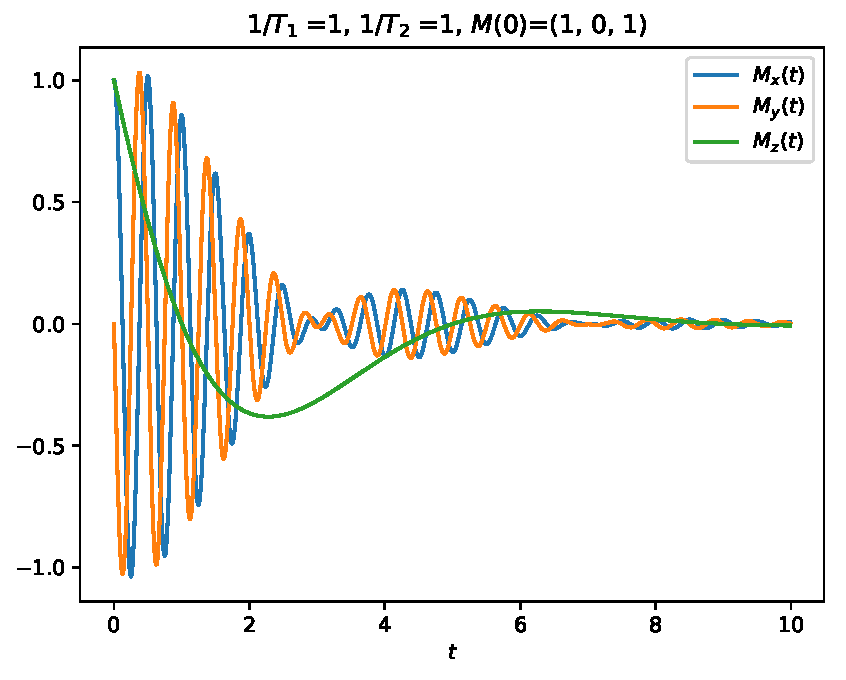
\includegraphics[width=2.5in]{figs/NMR_T1-1_T2-1_Minit-101_tau_0.01_t_10_phase_pi_2.pdf}
\caption{Time evolution of the bulk magnetization components for $1/T_1 = 1$, $1/T_2 = 1$, M(t=0) = (1, 0, 1), $\phi = \frac{\pi}{2}$}
\label{f15}
\end{figure}
\newpage

Results for phase $\phi = \frac{\pi}{4}, \frac{1}{T_1} = 0, \frac{1}{T_2} = 1$:
\begin{figure}[H]
\centering
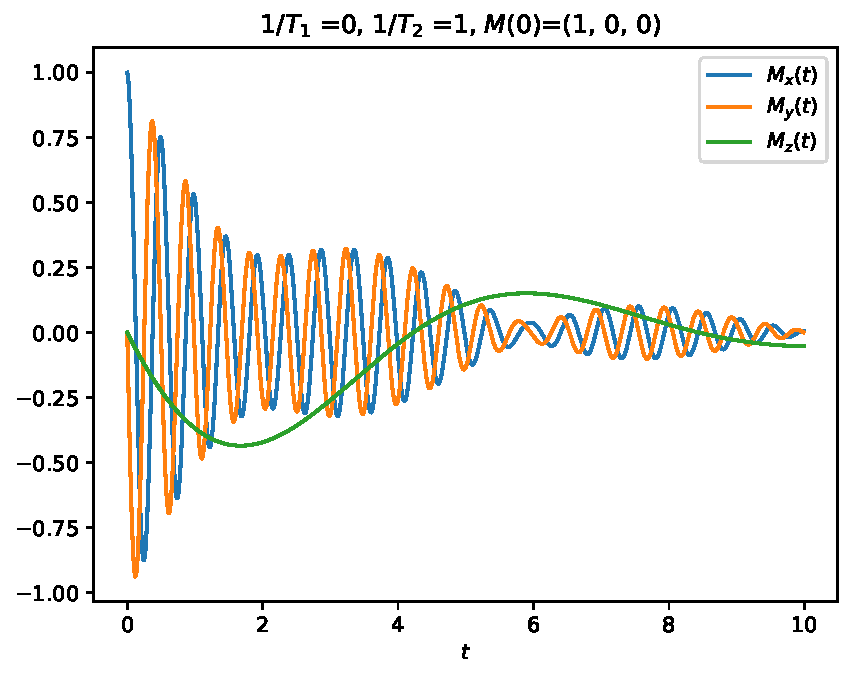
\includegraphics[width=2.5in]{figs/NMR_T1-0_T2-1_Minit-100_tau_0.01_t_10_phase_pi_4.pdf}
\caption{Time evolution of the bulk magnetization components for $1/T_1 = 0$, $1/T_2 = 1$, M(t=0) = (1, 0, 0), $\phi = \frac{\pi}{4}$}
\label{f16}
\end{figure}
\begin{figure}[H]
\centering
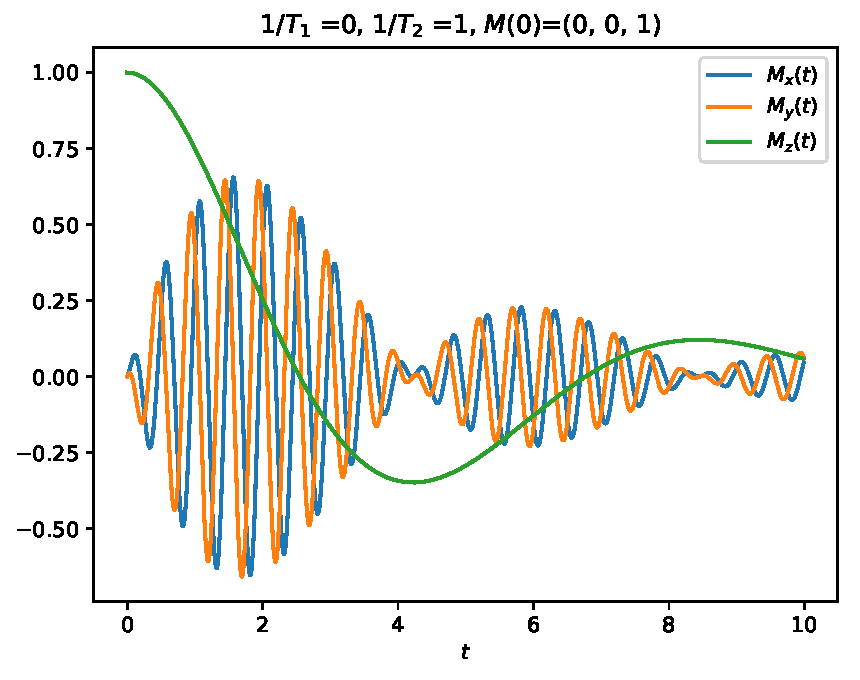
\includegraphics[width=2.5in]{figs/NMR_T1-0_T2-1_Minit-001_tau_0.01_t_10_phase_pi_4.pdf}
\caption{Time evolution of the bulk magnetization components for $1/T_1 = 0$, $1/T_2 = 1$, M(t=0) = (0, 0, 1), $\phi = \frac{\pi}{4}$}
\label{f17}
\end{figure}
\begin{figure}[H]
\centering
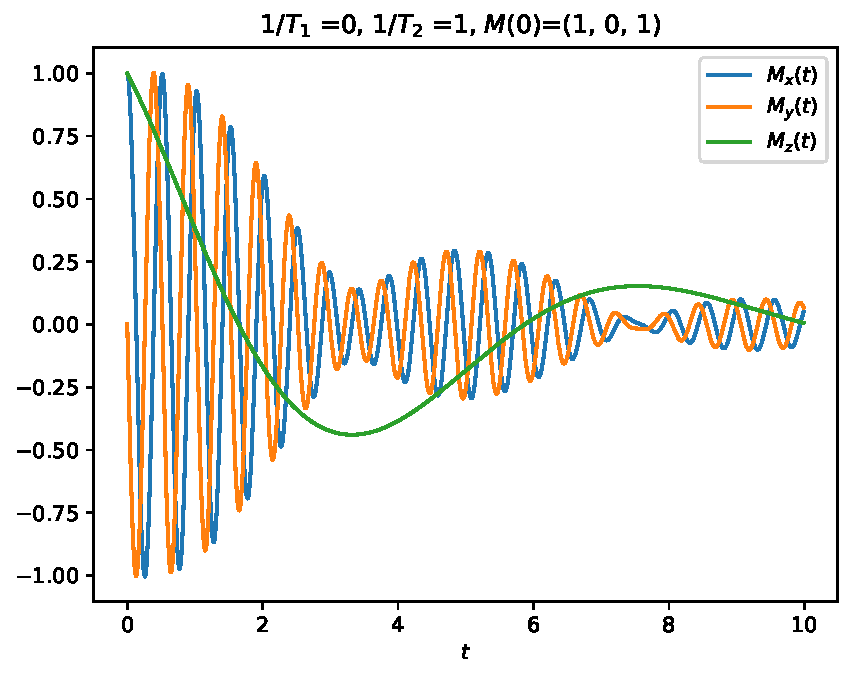
\includegraphics[width=2.5in]{figs/NMR_T1-0_T2-1_Minit-101_tau_0.01_t_10_phase_pi_4.pdf}
\caption{Time evolution of the bulk magnetization components for $1/T_1 = 0$, $1/T_2 = 1$, M(t=0) = (1, 0, 1), $\phi = \frac{\pi}{4}$}
\label{f18}
\end{figure}
\newpage

Results for phase $\phi = \frac{\pi}{4}, \frac{1}{T_1} = 1, \frac{1}{T_2} = 1$:
\begin{figure}[H]
\centering
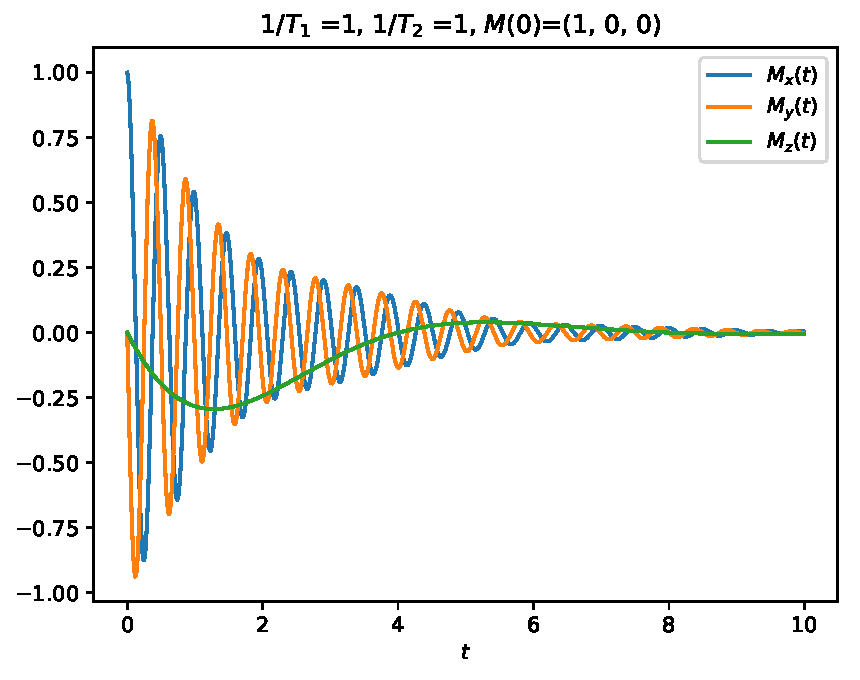
\includegraphics[width=2.5in]{figs/NMR_T1-1_T2-1_Minit-100_tau_0.01_t_10_phase_pi_4.pdf}
\caption{Time evolution of the bulk magnetization components for $1/T_1 = 1$, $1/T_2 = 1$, M(t=0) = (1, 0, 0), $\phi = \frac{\pi}{4}$}
\label{f19}
\end{figure}
\begin{figure}[H]
\centering
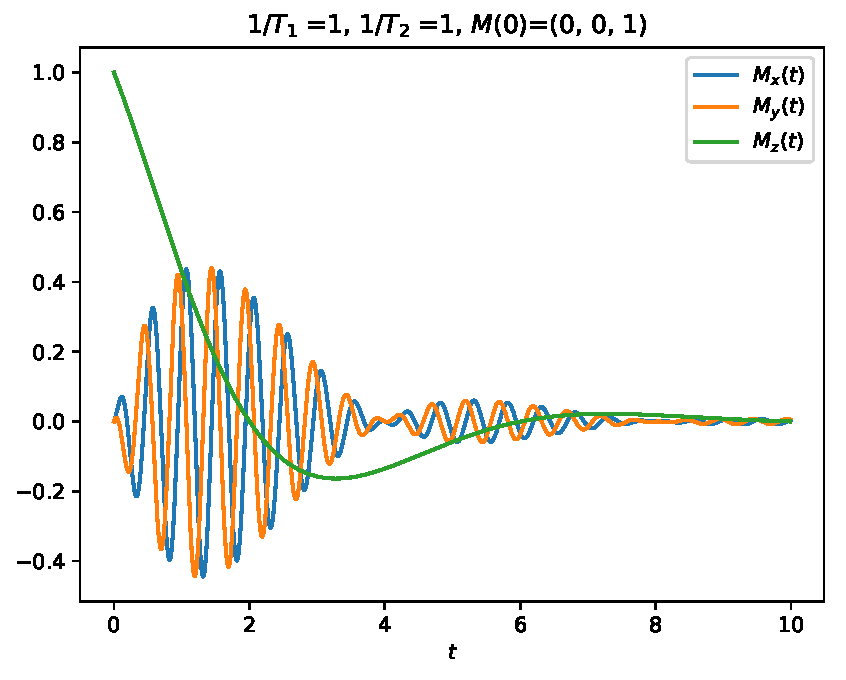
\includegraphics[width=2.5in]{figs/NMR_T1-1_T2-1_Minit-001_tau_0.01_t_10_phase_pi_4.pdf}
\caption{Time evolution of the bulk magnetization components for $1/T_1 = 1$, $1/T_2 = 1$, M(t=0) = (0, 0, 1), $\phi = \frac{\pi}{4}$}
\label{f20}
\end{figure}
\begin{figure}[H]
\centering
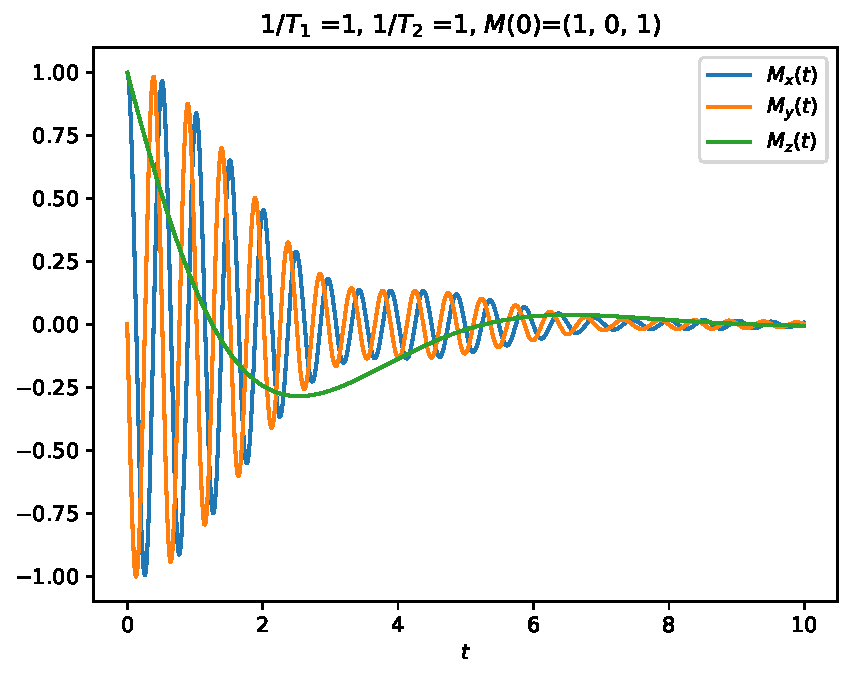
\includegraphics[width=2.5in]{figs/NMR_T1-1_T2-1_Minit-101_tau_0.01_t_10_phase_pi_4.pdf}
\caption{Time evolution of the bulk magnetization components for $1/T_1 = 1$, $1/T_2 = 1$, M(t=0) = (1, 0, 1), $\phi = \frac{\pi}{4}$}
\label{f21}
\end{figure}


\newpage
\onecolumn


\lstinputlisting{nmr_Toby.py}

\begin{thebibliography}{10}\footnotesize
%\bibitem{test} J. Appenzeller, J. Knoch, V. Derycke, R. Martel, S. Wind and Ph, Avouris, \lq\lq Field-modulated carrier transport in carbon nanotube transistors\rq\rq, {\it Phys. Rev. Lett.}, {\bf 89}, 126801 (2002).

\bibitem{Wessel} Prof. S. Wessel, Computational Physics, {\it Lecture Notes}
\bibitem{Michielsen} Prof. K. Michielsen, Computational Physics, {\it Lecture Notes}

\end{thebibliography}


%\bibliography{thesis_refs}
%\bibliographystyle{plain}




\end{document}